\documentclass[11pt, oneside]{article}
\usepackage[margin=1in]{geometry}
\geometry{letterpaper}
\usepackage{graphicx}
\usepackage{amssymb}
\usepackage[parfill]{parskip}
\usepackage{amssymb}
\usepackage{amsmath}
\usepackage{listings}
\usepackage{color}
\usepackage{standalone}
\usepackage{gensymb}
\usepackage{tikz}
\usetikzlibrary{matrix,chains,positioning,decorations.pathreplacing,arrows}
\usepackage{wrapfig}
\usepackage{epstopdf}
% \usepackage[outdir=./]{epstopdf}

\graphicspath{ {images/} }

\def\layersep{2.5cm}

\sloppy
\definecolor{lightgray}{gray}{0.5}
\setlength{\parindent}{0pt}
\definecolor{dkgreen}{rgb}{0,0.6,0}
\definecolor{gray}{rgb}{0.5,0.5,0.5}
\definecolor{mauve}{rgb}{0.58,0,0.82}

\lstset{frame=tb,
  language=Matlab,
  aboveskip=3mm,
  belowskip=3mm,
  showstringspaces=false,
  columns=flexible,
  basicstyle={\small\ttfamily},
  numbers=none,
  numberstyle=\tiny\color{gray},
  keywordstyle=\color{blue},
  commentstyle=\color{dkgreen},
  stringstyle=\color{mauve},
  breaklines=true,
  breakatwhitespace=true,
  tabsize=3
}

\title{Neuro 120 Homework 2: Data Analysis}
\author{William Schmitt and Will Drew}
\date{Due: Thursday 18 October 2018}

\begin{document}
\maketitle

\section{Question 1: Auditory Neuroplasticity}

\subsection{Raster Plot of Single-Unit Activity}

To plot the raster plot, we wrote the following code:
\lstinputlisting[firstline=5, lastline=23]{exposure_stimulus_investigation.m}
This produces the raster plot shown in Figure \ref{fig:RasterPlot}, which clearly shows that the neuron responds consistently to the stimulus about 0.03 seconds into the start of the trial.

\begin{figure}[ht!]
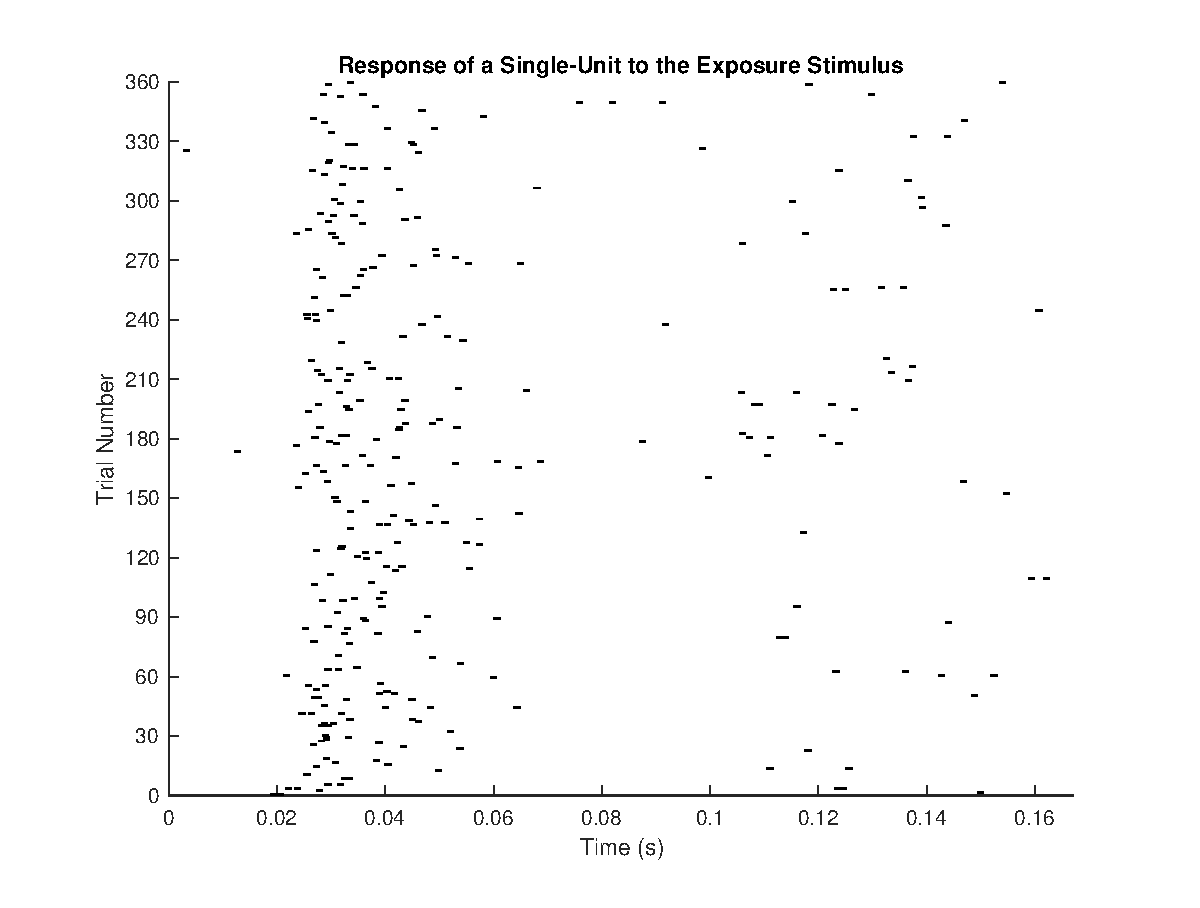
\includegraphics[width=1\textwidth]{RasterPlot.eps}
\caption{Raster Plot of Single-Unit Activity.}
\label{fig:RasterPlot}
\end{figure}

\subsection{Gaussian Kernel Firing Rate Estimate}

We calculate the estimate of the firing rate of this single-unit neuron by writing the following code:
\lstinputlisting[firstline=24, lastline=44]{exposure_stimulus_investigation.m}
This code simply places a Gaussian distribution with a standard deviation of 0.005s centered at the location of each spike and averages these distributions over all stimulus trials. This work produces Figure \ref{fig:Gaussian}, which shows that the firing rate increases dramatically around 0.03s into the trial, going from a baseline firing rate of about 5 Hz to a peak of just over 25 Hz.

\begin{figure}[ht!]
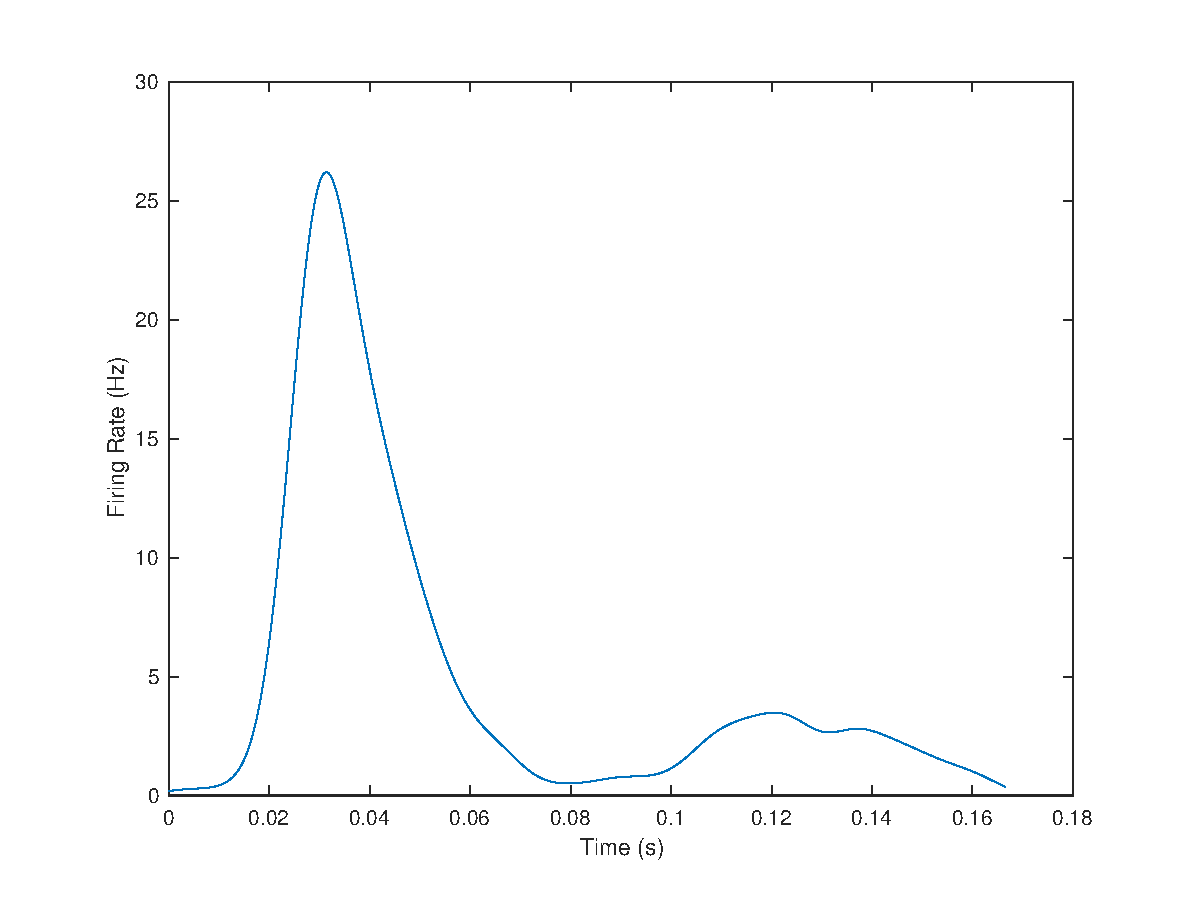
\includegraphics[width=1\textwidth]{fivemillisecondplot.eps}
\caption{Gaussian Estimation of Firing Rate Using $\sigma = 0.005s$.}
\label{fig:Gaussian}
\end{figure}

\subsection{Gaussian Kernel Parameter Variation}

We next alter the $\sigma$ parameter of the Gaussian kernel from above and generate Figures \ref{fig:point5ms} and \ref{fig:50ms} which shows the effect of this change. We used the following code to make these figures.
\lstinputlisting[firstline=46, lastline=68]{exposure_stimulus_investigation.m}
We can see from these figures that a very small standard deviation results in a quite noisy curve with large, quick oscillations, which intuitively, does not seem to describe the behavior of the neuron well as it is unlikely the firing rate would change that quickly. Conversely, a very large standard deviation results in a very smooth, wide curve that also does not seem to describe the data well as it predicts a large firing rate at the start of the experiment, where the raster plot indicates there is very little activity.

\begin{figure}[ht!]
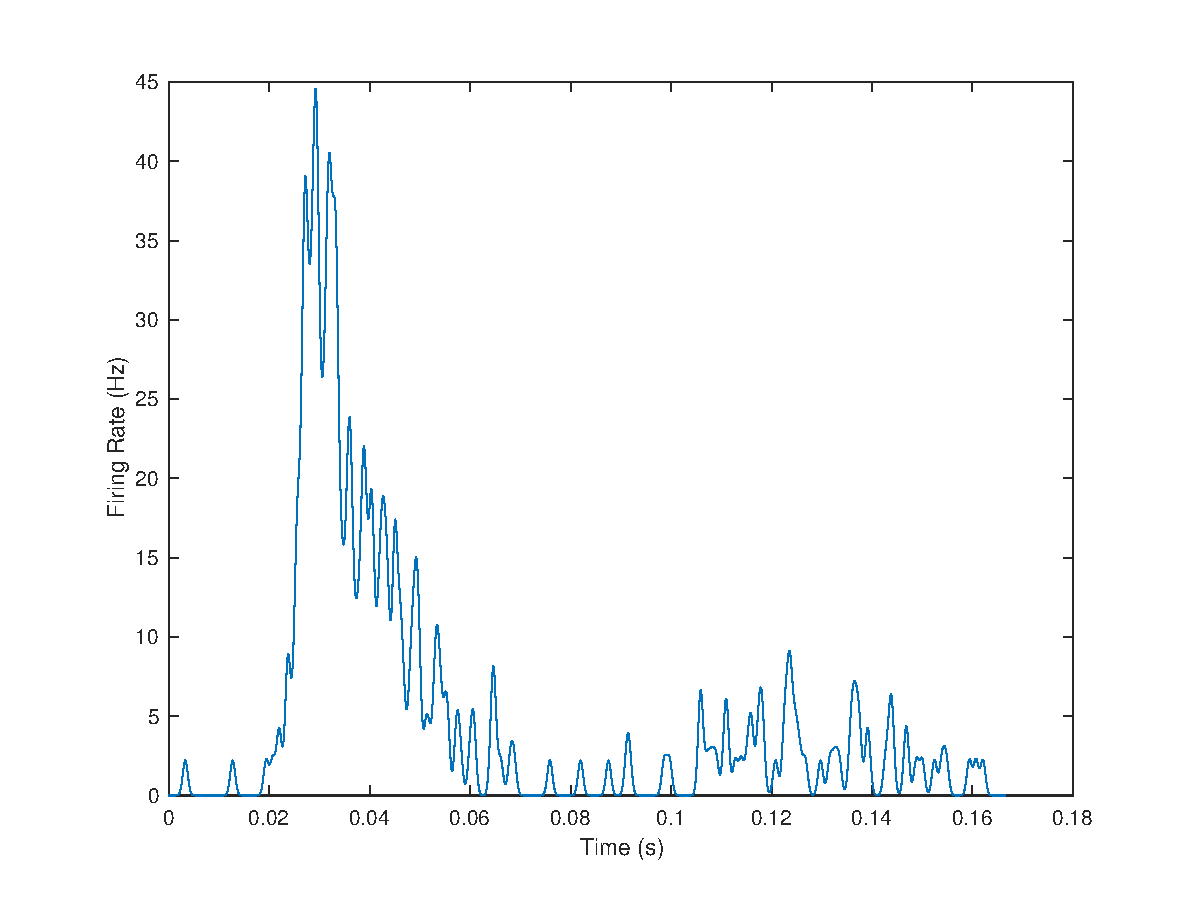
\includegraphics[width=1\textwidth]{halfmillisecondplot.eps}
\caption{Gaussian Estimation of Firing Rate Using $\sigma = 0.0005s$.}
\label{fig:point5ms}
\end{figure}


\begin{figure}[ht!]
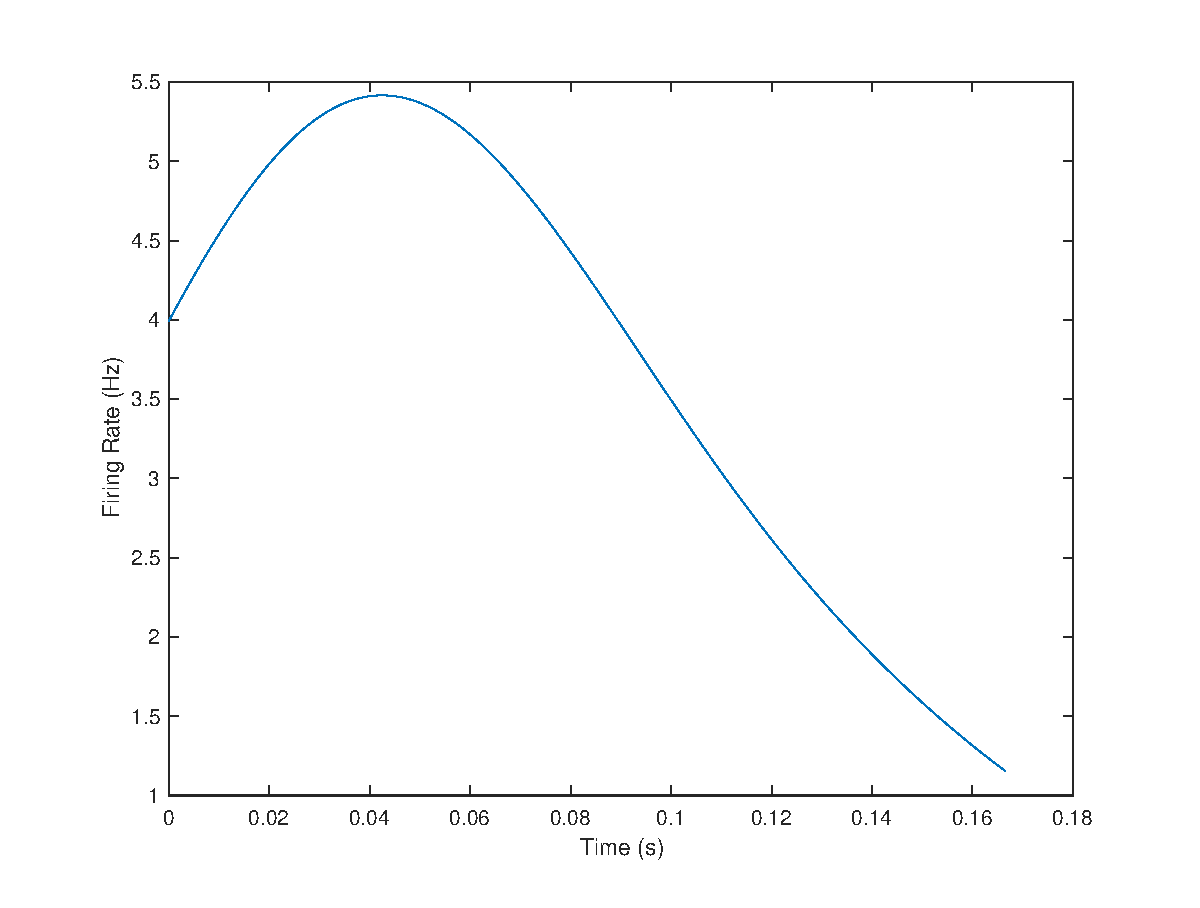
\includegraphics[width=1\textwidth]{fiftymillisecondplot.eps}
\caption{Gaussian Estimation of Firing Rate Using $\sigma = 0.05s$.}
\label{fig:50ms}
\end{figure}

\subsection{Grand Average Post-Stimulus Time Histogram}
We compute the grand average poststimulus time histogram using the following code:
\lstinputlisting[firstline=70, lastline=87]{exposure_stimulus_investigation.m}
This code generates Figure \ref{fig:PSTH}, which shows us the same trend we saw in the previous figures. The stimulus evokes a larger response from the population of neurons about 0.03 seconds after the onset of a trial.

\begin{figure}[ht!]
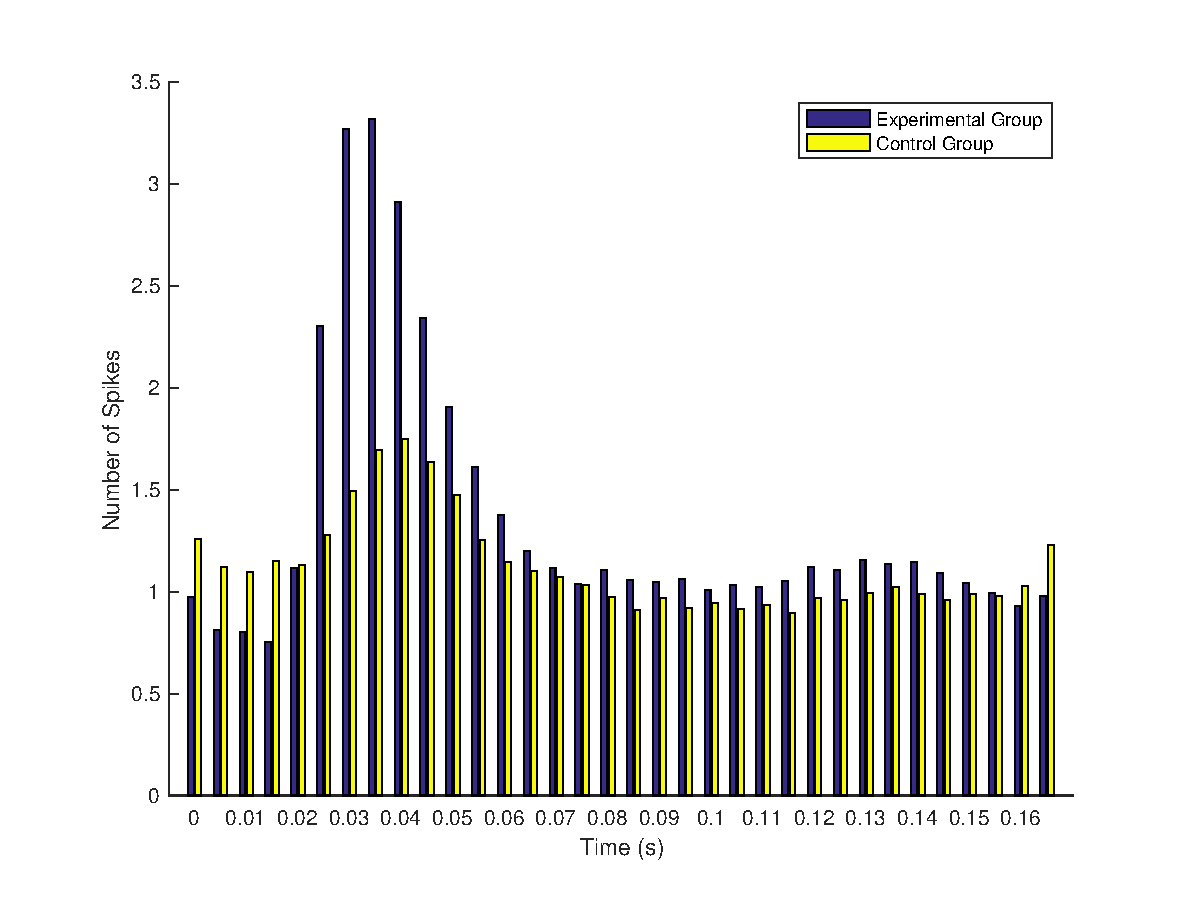
\includegraphics[width=1\textwidth]{Q1PD.eps}
\caption{Grand Average Post-Stimulus Time Histogram of two Populations of Neurons. Bin width was 5ms.}
\label{fig:PSTH}
\end{figure}

\subsection{Differences between Experimental and Control Groups}

Looking at Figure \ref{fig:PSTH}, we see that the experimental group has a stronger response (i.e. more spikes)
during the peak firing activity (about 0.02s to 0.05s after the onset of the trial) of the neurons. However, the control neuron population still exhibits this increase, so therefore it is just that the experimental group of neurons became more selective to the exposure stimulus while the precision of the response did not appear to change. Finally, we can see that there is very little difference in the activity of the two groups (beyond some higher activity in the control group at the start and end of a trial) outside of this peak firing range.

\subsection{Spike-Triggered Average for Neuron}

\subsection{Frequency Selectivity of Neuron}

\subsection{Neuronal Stimulus Preference}

\subsection{Potential Stimulus Correlations}

\section{Random Neural Networks and Overfitting in Regression}

\subsection{Linear Regression with Regularization}

We implement linear regression with regularization in Matlab as follows:
\lstinputlisting[firstline=1, lastline=59]{nn_regression.m}
This produces Figure \ref{fig:regression} which shows us how this network performs on test data. We see from this data that the 26 neuron model performed the best (as measured by mean squared error and visual inspection of the curve it makes), while the 10 neuron model performed reasonably well, but with some more error. Finally, the 2 neuron model performed the worst of all and has quite the large error.

\begin{figure}[ht!]
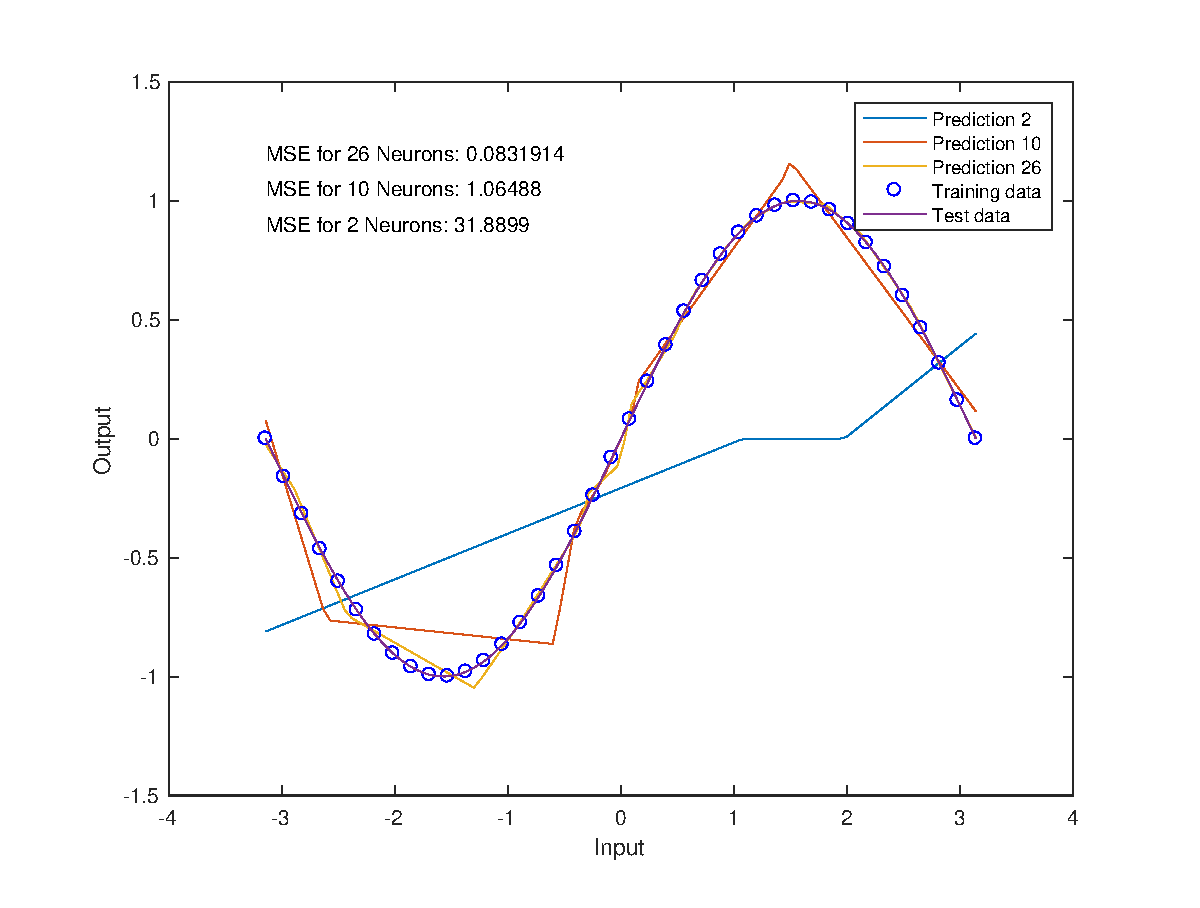
\includegraphics[width=1\textwidth]{Q2PartA.eps}
\caption{Performance of Simple Linear Regression with varying numbers of neurons}
\label{fig:regression}
\end{figure}

\subsection{Overdetermined Networks}

We implement the overdetermined network scenario as follows:
\lstinputlisting[firstline=61, lastline=108]{nn_regression.m}
This code produces Figure \ref{fig:overdetermined}, which shows us what happens in the overdetermined network scenario. We see from this figure that the network is quite unstable throughout this size range. Indeed, the mean squared error is quite low for networks with less than 10 neurons, 15 neurons, or 25 neurons. However, the mean squared error is astronomically high for values close to this: networks with 12, 21, and 22 neurons. Thus, we see that when the model is too small, the mean squared error might be low, but the predictions don't map neatly onto the ``ideal'' function we are approximating (as seen in Figure \ref{fig:regression}). However, when the model is too big, the mean squared error is quite large and the model likely fits the data too well such that it cannot generalize to new test data.

\begin{figure}[ht!]
\includegraphics[width=1\textwidth]{Q2PartB.eps}
\caption{Mean-Squared Error as a Function of Network Size for the Over-Determined Situation.}
\label{fig:overdetermined}
\end{figure}

\subsection{Underdetermined Networks}

We implement the underdetermined network scenario as follows:
\lstinputlisting[firstline=110, lastline=157]{nn_regression.m}
This code produces Figure \ref{fig:underdetermined}, which we see produces a low mean-squared error for large network sizes. Thus, based on this figure, we would guess that the best network size is approximately 110 neurons or so (as the mean squared error seems to plateau after this). The performance of these big networks is not as variable as the smaller networks.

\begin{figure}[ht!]
\includegraphics[width=1\textwidth]{Q2PartC.eps}
\caption{Mean-Squared Error as a Function of Network Size for the Under-Determined Situation.}
\label{fig:underdetermined}
\end{figure}

\subsection{Label Noise and Regularization Parameters}

\subsection{Reflections}

\section{Image Demixing}

\subsection{Covariance Matrix and PCA}

\subsubsection{De-meaning the data}

\subsubsection{Covariance Matrix Function}

\subsubsection{Eigenvectors and values of covariance matrix}

\subsubsection{Time Required for Computation}

\subsection{Whitening the Data}

\subsection{ICA}

\subsubsection{Mixed Images}

\subsubsection{Whitening mixed images}

\subsubsection{Results of ICA}





\end{document}
